\chapter{Ocena eksperymentalna}
\section{Cel Badań}
Celem badań było sprawdzenie jak popularne algorytmy uczenia maszynowego radzą sobie z rozwiązaniem problemu 
klasyfikacji informacji jako prawdziwe lub nieprawdziwe. W celu sprawdzenia ich efektywności należało zbadać
takie cechy jak:
\begin{itemize}
    \item czas fazy uczenia,
    \item czas fazy predykcji,
    \item procent poprawnych predykcji po nauczeniu modelu.
\end{itemize}
W badaniach głównym sprawdzanym elementem było to, jak zmiana długości NGramów, na które podzielony
został tekst przed wektoryzacją wpływa na wyniki algorytmów i odnalezienie takiego rozmiaru, który
daje najlepsze wyniki. 

Do badania wybrano pięć popularnych algorytmów uczenia maszynowego: 
\begin{itemize}
    \item KNN - K najbliższych sąsiadów,
    \item SVM - maszyna wektorów nośnych,
    \item Naive Bayes,
    \item Random forest - las losowy,
    \item MLP - wielowarstwowy perceptron.
\end{itemize} 
\section{Warunki przeprowadzonego eksperymentu}
Badania zostały wykonane na komputerze stacjonarnym o następującej specyfikacji:
\begin{itemize}
    \item system operacyjny Windows 10 Pro w wersji 10.0.19041,
    \item procesor AMD Ryzen 5 3600,
    \item pamięć RAM 16 GB.
\end{itemize}
Wszystkie badania były wykonywane w jednakowych warunkach, aby można było 
je w prosty sposób porównywać. 

Dane badawcze to zbiór pod nazwą ``ISOT Fake News Dataset'' przygotowany przez uczelnię w 
Kanadzie ``Univerity of Victoria''. Zawiera on 12600 artykułów prawdziwych pochodzących ze strony
internetowej Reuters.com oraz 12600 artykułów nieprawdziwych zebranych z niewiarygodnych źródeł
oznaczonych przez organizację do sprawdzania faktów Politifact. Tematyka artykułów to głównie polityka i wiadomości 
ze świata.  Teksty zawarte w zbiorze zostały wstępnie przygotowane, jednak błędy znajdujące się w nieprawdziwych 
artykułach pozostały. Zbiór został pobrany w dniu 16 czerwca 2020 z witryny znajdującej się pod adresem \url{https://www.uvic.ca/}.~\cite{ISOT}

Algorytmy KNN, Random forest oraz Naive Bayes zostały zbadane na rozmiarach NGramów od 1 do 10, natomiast
MLP i SVC od 1 do 5 z powodu dużej złożoności obliczeniowej przy większym rozmiarze. Podczas
dzielenia danych na treningowe i testowe został wykorzystany parametr random\_state, który gwarantuje
że dane zostaną zawsze podzielone w jednakowy sposób.
\section{Wyniki}
W opisanych poniżej wynikach, każdy z algorytmów został zbadany pod kątem trzech cech. 
Efektywność została zmierzona funkcją \textit{``Score''} na 40\% danych ze zbioru.
\begin{table}[H]
    \centering
    \caption{Wyniki algorytmu KNN wektoryzacja metodą Bag of words}
    \resizebox{\textwidth}{!}{%
    \begin{tabular}{ | l | c | c | c | c | c | c | c | c | c | c |}
        \hline
        Rozmiar Ngramu & 1 & 2 & 3 & 4 & 5 & 6 & 7 & 8 & 9 & 10  \\ \hline
        Efektywność & 75.65\% & 84.36\% & 63.52\% & 48.93\% & 47.5\% & 47.24\% & 47.23\% & 47.41\% & 61.48\% & 53.81\%  \\ \hline
        Czas fazy uczenia & 0.003s & 0.022s & 0.059s & 0.099s & 0.102s & 0.121s & 0.126s & 0.129s & 0.122s & 0.129s  \\ \hline
        Czas fazy predykcji & 27.221s & 180.565s & 312.157s & 221.672s & 137.788s & 91.407s & 67.833s & 54.803s & 45.88s & 40.02s  \\ \hline
    \end{tabular}
    }
\end{table}

\begin{table}[H]
    \centering
    \caption{Wyniki algorytmu KNN wektoryzacja metodą TFIDF}
    \resizebox{\textwidth}{!}{%
    \begin{tabular}{ | l | c | c | c | c | c | c | c | c | c | c |}
        \hline
        Rozmiar Ngramu & 1 & 2 & 3 & 4 & 5 & 6 & 7 & 8 & 9 & 10  \\ \hline
        Efektywność & 78.13\% & 71.26\% & 60.09\% & 64.01\% & 47.7\% & 47.54\% & 53.89\% & 53.66\% & 53.64\% & 53.63\%   \\ \hline
        Czas fazy uczenia & 0.003s & 0.024s & 0.067s & 0.092s & 0.112s & 0.111s & 0.122s & 0.123s & 0.127s & 0.129s \\ \hline
        Czas fazy predykcji & 27.168s & 186.84s & 321.7s & 220.716s & 141.115s & 93.327s & 68.613s & 46.536s & 47.467s & 37.644s  \\ \hline
    \end{tabular}
    }
\end{table}

\begin{table}[H]
    \centering
    \caption{Wyniki algorytmu Random Forest wektoryzacja metodą Bag of words}
    \resizebox{\textwidth}{!}{%
    \begin{tabular}{ | l | c | c | c | c | c | c | c | c | c | c |}
        \hline
        Rozmiar Ngramu & 1 & 2 & 3 & 4 & 5 & 6 & 7 & 8 & 9 & 10 \\ \hline
        Efektywność & 84.15\% & 98.09\% & 99.59\% & 99.81\% & 99.64\% & 99.33\% & 99.05\% & 98.81\% & 98.59\% & 98.29\%  \\ \hline
        Czas fazy uczenia & 23.56s & 47.484s & 48.267s & 45.867s & 52.639s & 73.57s & 108.591s & 143.566s & 187.709s & 225.265s \\ \hline
        Czas fazy predykcji & 0.234s & 0.764s & 2.587s & 5.095s & 6.324s & 8.315s & 15.628s & 19.665s & 23.49s & 25.823s  \\ \hline
    \end{tabular}
    }
\end{table}

\begin{table}[H]
    \centering
    \caption{Wyniki algorytmu Random Forest wektoryzacja metodą TFIDF}
    \resizebox{\textwidth}{!}{%
    \begin{tabular}{ | l | c | c | c | c | c | c | c | c | c | c |}
        \hline
        Rozmiar Ngramu & 1 & 2 & 3 & 4 & 5 & 6 & 7 & 8 & 9 & 10 \\ \hline
        Efektywność & 83.43\% & 98.15\% & 99.54\% & 99.82\% & 99.55\% & 99.27\% & 99.0\% & 98.62\% & 98.68\% & 98.24\%  \\ \hline
        Czas fazy uczenia & 26.536s & 57.014s & 53.246s & 47.681s & 48.82s & 63.392s & 92.896s & 132.436s & 175.463s & 217.02s \\ \hline
        Czas fazy predykcji & 0.24s & 0.729s & 3.027s & 5.021s & 6.554s & 7.893s & 14.047s & 20.172s & 24.588s & 26.493s  \\ \hline
    \end{tabular}
    }
\end{table}

\begin{table}[H]
    \centering
    \caption{Wyniki algorytmu Naive Bayes wektoryzacja metodą Bag of words}
    \resizebox{\textwidth}{!}{%
    \begin{tabular}{ | l | c | c | c | c | c | c | c | c | c | c |}
        \hline
        Rozmiar Ngramu & 1 & 2 & 3 & 4 & 5 & 6 & 7 & 8 & 9 & 10 \\ \hline
        Efektywność & 69.53\% & 78.91\% & 83.96\% & 92.19\% & 94.92\% & 96.12\% & 96.54\% & 96.67\% & 96.5\% & 96.29\%  \\ \hline
        Czas fazy uczenia & 0.005s & 0.031s & 0.102s & 0.147s & 0.201s & 0.377s & 0.551s & 0.692s & 0.837s & 1.027s \\ \hline
        Czas fazy predykcji & 0.003s & 0.016s & 0.047s & 0.072s & 0.095s & 0.182s & 0.299s & 0.362s & 0.382s & 0.41s  \\ \hline
    \end{tabular}
    }
\end{table}

\begin{table}[H]
    \centering
    \caption{Wyniki algorytmu Naive Bayes wektoryzacja metodą TFIDF}
    \resizebox{\textwidth}{!}{%
    \begin{tabular}{ | l | c | c | c | c | c | c | c | c | c | c |}
        \hline
        Rozmiar Ngramu & 1 & 2 & 3 & 4 & 5 & 6 & 7 & 8 & 9 & 10 \\ \hline
        Efektywność & 75.19\% & 81.98\% & 85.54\% & 92.43\% & 94.78\% & 96.11\% & 96.58\% & 96.71\% & 96.56\% & 96.38\%  \\ \hline
        Czas fazy uczenia & 0.005s & 0.033s & 0.105s & 0.159s & 0.193s & 0.293s & 0.504s & 0.675s & 0.853s & 1.02s \\ \hline
        Czas fazy predykcji & 0.002s & 0.017s & 0.05s & 0.077s & 0.09s & 0.145s & 0.319s & 0.343s & 0.406s & 0.407s  \\ \hline
    \end{tabular}
    }
\end{table}

\begin{table}[H]
    \centering
    \caption{Wyniki algorytmu SVC wektoryzacja metodą Bag of words}
    \begin{tabular}{ | l | c | c | c | c | c |}
        \hline
        Rozmiar Ngramu & 1 & 2 & 3 & 4 & 5 \\ \hline
        Efektywność & 81.36\% & 96.1\% & 97.75\% & 98.45\% & 98.34\%   \\ \hline
        Czas fazy uczenia & 14.175s & 319.6s & 2779.462s & 7282.055s & 10144.174s  \\ \hline
        Czas fazy predykcji & 8.18s & 127.618s & 716.666s & 1502.585s & 2534.03s  \\ \hline
    \end{tabular}
\end{table}

\begin{table}[H]
    \centering
    \caption{Wyniki algorytmu SVC wektoryzacja metodą TFIDF}
    \begin{tabular}{ | l | c | c | c | c | c |}
        \hline
        Rozmiar Ngramu & 1 & 2 & 3 & 4 & 5   \\ \hline
        Efektywność & 79.47\% & 96.61\% & 97.95\% & 98.65\% & 98.66\% \\ \hline
        Czas fazy uczenia & 14.046s & 220.009s & 3068.672s & 8322.766s & 10384.898s \\ \hline
        Czas fazy predykcji & 8.008s & 106.538s & 751.689s & 1594.27s & 2286.608s  \\ \hline
    \end{tabular}
\end{table}

\begin{table}[H]
    \centering
    \caption{Wyniki algorytmu MLP wektoryzacja metodą Bag of words}
    \begin{tabular}{ | l | c | c | c | c | c |}
        \hline
        Rozmiar Ngramu & 1 & 2 & 3 & 4 & 5  \\ \hline
        Efektywność & 81.68\% & 97.16\% & 98.6\% & 97.79\% & 98.37\%   \\ \hline
        Czas fazy uczenia & 32.655s & 22.982s & 115.108s & 544.161s & 2038.845s  \\ \hline
        Czas fazy predykcji & 0.039s & 0.11s & 0.373s & 1.085s & 2.444s  \\ \hline
    \end{tabular}
\end{table}

\begin{table}[H]
    \centering
    \caption{Wyniki algorytmu MLP wektoryzacja metodą TFIDF}
    \begin{tabular}{ | l | c | c | c | c | c |}
        \hline
        Rozmiar Ngramu & 1 & 2 & 3 & 4 & 5   \\ \hline
        Efektywność & 79.8\% & 97.43\% & 98.6\% & 98.69\% & 98.09\%   \\ \hline
        Czas fazy uczenia & 16.176s & 22.159s & 111.424s & 520.082s & 1926.648s  \\ \hline
        Czas fazy predykcji & 0.034s & 0.113s & 0.38s & 0.911s & 2.133s  \\ \hline
    \end{tabular}
\end{table}
\section{Analiza wyników wraz z oceną statystyczną}

\begin{figure}[h!]
    \centering
    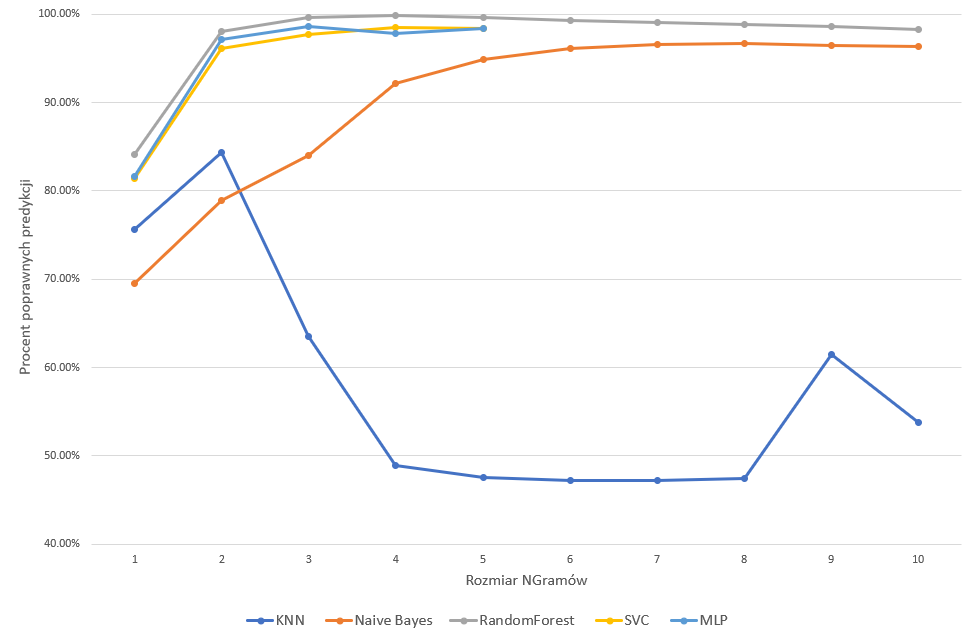
\includegraphics[width=0.9\textwidth]{./Img/BOWAcc.png}
    \caption{Efektywność algorytmów wektoryzacja metodą Bag of words}
\end{figure}

\begin{figure}[h!]
    \centering
    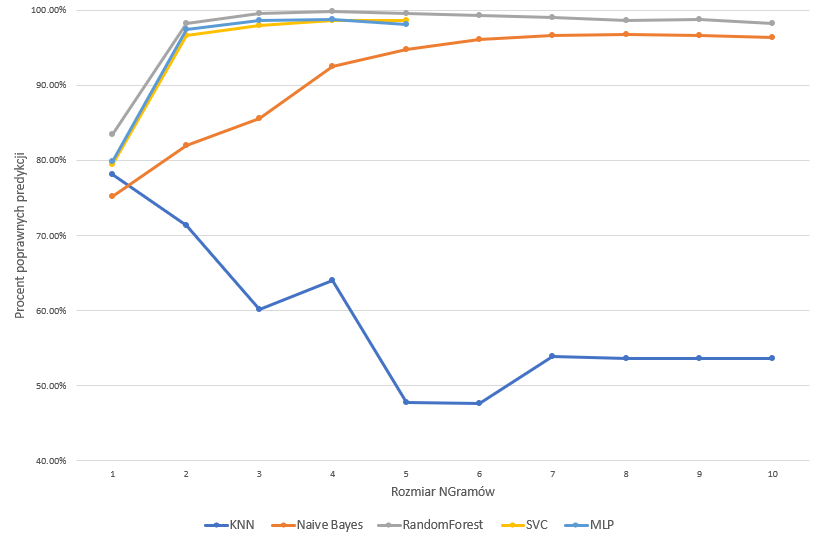
\includegraphics[width=0.9\textwidth]{./Img/TFIDFAcc.png}
    \caption{Efektywność algorytmów wektoryzacja metodą TFIDF}
\end{figure}

\begin{figure}[h!]
    \centering
    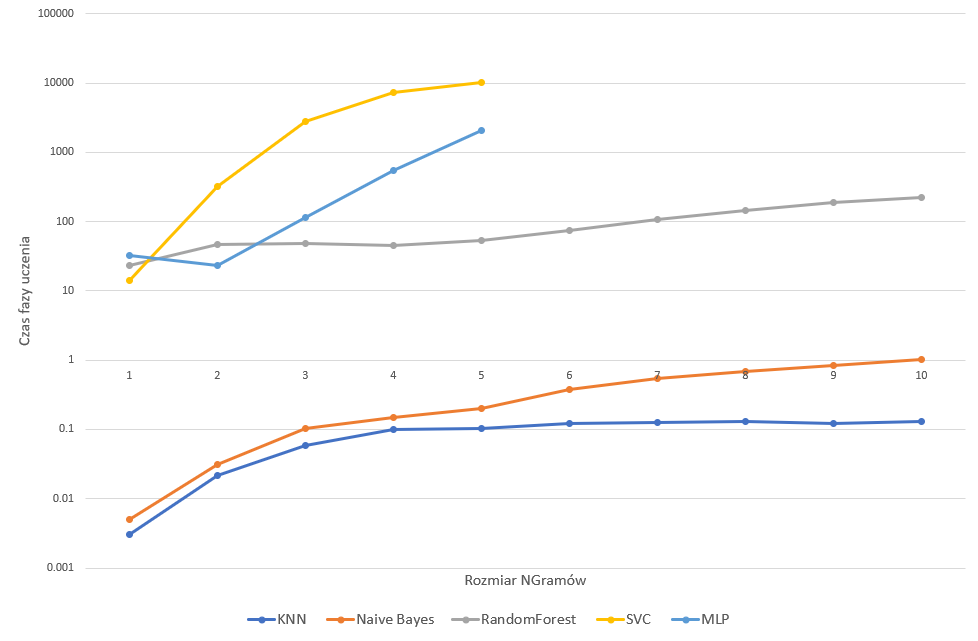
\includegraphics[width=0.9\textwidth]{./Img/BOWLearn.png}
    \caption{Czasy uczenia algorytmów}
\end{figure}

\begin{figure}[h!]
    \centering
    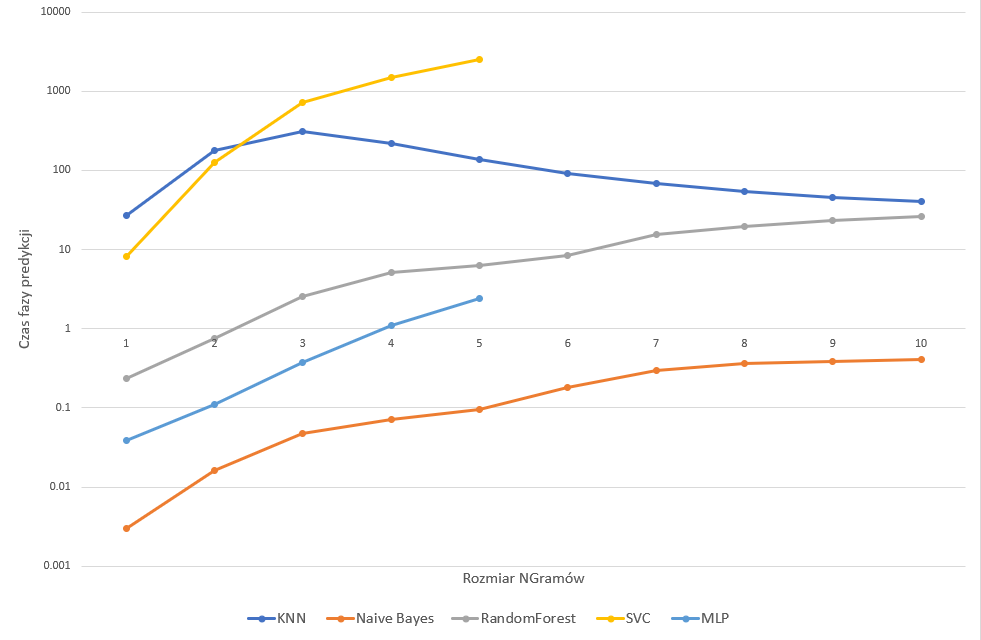
\includegraphics[width=0.9\textwidth]{./Img/BOWPredict.png}
    \caption{Czasy predykcji algorytmów}
\end{figure}

Wyniki zostały przeanalizowane pod kątem trzech badanych cech:

\begin{itemize}
    \item Efektywność
    
    Pod względem efektywności algorytmy sprawdziły się następująco:
    \begin{itemize}
        \item KNN -
        dla długości równej 1 algorytm osiąga wyniki większe od 70\%, jednak wraz 
        z podnoszeniem się jej zmniejsza się także efektywność. W przypadku obu metod 
        wektoryzacji rozmiary 5 i 6 dają wyniki poniżej 50\%, co oznacza, że są one gorsze 
        od predykcji wykonanej na podstawie rzutu monetą. Jest to związane 
        z overfittingiem będącym skutkiem podnoszenia się ilości cech. Najlepszym wynikiem w 
        przypadku KNN jest 84.36\% przy wykorzystaniu metody wektoryzacji Bag of words i rozmiarze równym 2,
        a najgorszym 47.5\%  przy wykorzystaniu metody Bag of words i rozmiaru 5,

        \item Random forest, SVC, MLP -        
        algorytmy te zachowują się w bardzo podobny sposób. Zwiększanie długości NGramów 
        do wartości 4 powoduje bardzo szybki wzrost efektywności do nawet 99.82\%, natomiast zmiana 
        długości ponad 4 prowadzi do powolnego spadku możliwości predykcyjnych, co może być 
        związane podobnie jak w przypadku algorytmu KNN z overfittingiem. Algorytmy te osiągają najlepsze 
        wyniki pod względem efektywności ze wszystkich badanych,
        \item Naive Bayes -
        Algorytm Naive Bayes zwiększa swoją efektywność w taki sposób jak Random Forest, SVC oraz MLP 
        jednak robi to dużo wolniej i osiąga swoją szczytową efektywność dla długości równej 8 przy której 
        jest ona równa 96.56\%. Dalsze wydłużanie NGramów prowadzi do powolnego spadku możliwości predykcyjnych.
        Algorytm Naive Bayes osiąga najniższe wyniki w przypadku podziału na NGramy o długości równej 1, gdzie 
        poprawnie klasyfikuje tylko 69.63\% danych testowych.
    \end{itemize}
    \item Czasy fazy uczenia
    
    Pod względem czasu fazy uczenia algorytmy sprawdziły się następująco:
    
    \begin{itemize}
        \item KNN, Naive Bayes -
        Algorytmy KNN oraz Naive Bayes osiągnęły najlepsze wyniki czasu trwania fazy uczenia, która podczas 
        trwania całego badania nie była dłuższa niż jedna sekunda.
        Jest to spowodowane względnie prostymi operacjami wykonywanymi przez nie podczas tej fazy. 
        Zadaniem algorytmu KNN jest jedynie zapisanie wszystkich danych, natomiast Naive Bayes  
        oblicza prawdopodobieństwa na podstawie prostych kalkulacji wykonywanych podczas jednej iteracji,
        \item Random forest -
        czas trwania fazy uczenia dla algorytmu Random Forest ulega niewielkiemu wydłużaniu podczas zmiany rozmiaru 
        NGramów, jednak podczas całego badania jest on przeciętny, przez co nie trwa zbyt długo, ale też nie jest szybki.
        Faza ta w tym przypadku polega na stworzeniu drzewa decyzyjnego jak najlepiej podejmującego decyzje. Czas ten nie
        ulega znacznemu wydłużeniu przy większej liczbie cech, ponieważ algorytm wybiera tylko najważniejsze z nich do stworzenia 
        drzewa,
        \item SVC, MLP -
        w przypadku obu tych algorytmów można zauważyć znacznie zwiększanie się czasu uczenia wraz ze zwiększaniem
        długości NGramów. Doprowadziło to w ich przypadku do ograniczenia badań tylko do długości równej 5,
        ponieważ czas tej fazy wynosił niemal 3 godziny. Takie wyniki powodują, że nieprawdopodobne jest 
        ich efektywne wykorzystanie w systemach rozpoznawania fake newsów. 
    \end{itemize}
    \item Czasy fazy predykcji
    
    Pod względem czasu fazy predykcji algorytmy sprawdziły się następująco:
    
    \begin{itemize}
        \item KNN -
        predykcja tego algorytmu jest znacznie dłuższa niż uczenia i dla mniejszych długości NGramów trwa
        najdłużej. Początkowo zwiększanie długości powoduje wzrost czasu, jednak po osiągnięciu maksimum dla rozmiaru 3
        następuje powolna stabilizacja w kierunku około 40 sekund,
        \item Random forest -
        czas trwania fazy predykcji zwiększa się powoli do wartości 26.49 sekund. Spowodowane jest to zwiększaniem
        się drzewa decyzyjnego który jest trawersowany w celu podjęcia decyzji. Czas ten podobnie jak w przypadku 
        fazy uczenia jest przeciętny w porównaniu z innymi algorytmami,
        \item Naive Bayes -
        Jest to najszybszy algorytm zarówno pod względem fazy uczenia, jak i predykcji, której wykonanie 
        opiera się na wyliczeniu odpowiednich prawdopodobieństw będących dla maszyny bardzo prostym zadaniem,
        \item SVC -
        czas trwania fazy predykcji jest bardzo podobny do czasu uczenia. Użycie SVC trwa zbyt długo
        by mógł on być zaimplementowany w jakichkolwiek systemach,
        \item MLP -
        w porówaniu z fazą uczenia predykcja następuje bardzo szybko, ponieważ opiera się tylko
        na aktywacji odpowiednich neuronów w stworzonym wcześniej modelu. Jest on na drugim miejscu
        pod względem prędkości wykonywania predykcji.
    \end{itemize}
\end{itemize}




\section{Wnioski z badań}
Przeprowadzone badania pozwoliły na odnalezienie odpowiedzi na pytanie 
będące celem niniejszej pracy. Wykorzystanie algorytmów uczenia maszynowego 
w rozpoznawaniu fałszywych informacji skutkuje osiągnięciem bardzo optymistycznych wyników.
Z badanych w algorytmów jedynie algorytm KNN swoją efektywnością dla 
każdej długości NGramów nie pozwoliłby na pewne podjęcie decyzji, czy dany artykuł jest prawdziwy, czy też nie.
Może to być związane z bardzo dużą ilością cech w tekście, co bardzo szybko prowadzi do tak zwanego 
overfittingu. 

Z powodu eksponencjalnego zwiększania się ilości cech wraz ze zwiększaniem długości NGramów, 
algorytmy takie jak SVC oraz MLP osiągają już dla długości równej 5 zbyt długie czasy trwania faz uczenia sięgające 
do 3 godzin. Czas taki nie pozwala na wykorzystanie ich w systemach detekcji fake newsów, ponieważ
musiałyby one analizować dużą ilość artykułów, dla których bardzo duże znaczenie ma to jak 
szybko pojawią się na docelowej stronie internetowej bądź mediach społecznościowych.

Najlepszym z algorytmów okazał się Random Forest, który dla NGramów o długości równej 4
osiągnął efektywność równą 99.82\%. Pomimo iż efektywność ta została prawie osiągnięta przez algorytmy
SVC oraz MLP to były one znacznie wolniejsze podczas fazy uczenia, a także podczas fazy 
predykcji w przypadku SVC. Szybszy od Random Forest algorytm Naive Bayes również osiągnął zadowalające wyniki,
jednak w przypadku Fake Newsów najbardziej znacząca jest efektywność, której nawet niewielki deficyt
może być katastrofalny w skutkach.  

Zauważono także, że wybór metody wektoryzacji ma niewielki wpływ na to jak dobrze wykorzystany algorytm 
sprawdzi się w wykonywaniu swojego zadania. Jeżeli chodzi o czas trwania poszczególnych faz to 
różnica w czasie wynosiła zazwyczaj poniżej paru sekund w przypadku dłuższych algorytmów lub poniżej 
sekundy w przypadku krótszych. Pod względem efektywności można także zauważyć niewielkie różnice,
które przeplatają się
wraz ze zmianą długości, z tego powodu nie jest możliwe określenie, która metoda jest lepsza.

Wykorzystanie technologii machine learningu do zadania detekcji Fake Newsów 
może stanowić rozwiązanie problemów jakie niosą ze sobą fałszywe informacje. Ich automatyczna 
detekcja uchroniłaby miliony ludzi przed byciem oszukanym. 
